%%%%%%%%%%%%%%%%
%\chapter{Language Restrictions (Main Result: Theorems)}
%%%%%%%%%%%%%%%%

%State clearly definitions, assumptions, and proofs. The document will be archived for posterity and your name will be associated with any mistakes you make.

%%%%%%%%%%%%%%%%%%%%%%%%%%%%%%%%
\chapter{Design}
%%%%%%%%%%%%%%%%%%%%%%%%%%%%%%%%
% Introduce and discuss the design decisions that you made during this project.
% Highlight why individual decisions are important and/or necessary. Discuss
% how the design fits together.
% Use as much as needed.

The goal is to port Java to native restrictions with a minimal set of changes to the JDK. We want Java to behave exactly like Native Image, and crash for the exact same reasons that Native Image does. 
This section explains how semantic changes can be modeled through the concept of (1) native restrictions, (2) how defining scopes in the JDK enables us to express these changes, and (3) how we can improve Native Image usability by improving the turnaround for computing reachability metadata, by facilitating debugging of user code and defining the expected behaviour of Native Image.

%%%%%%%%%%%%%%%%%%%%%%%%%%%%%%%%
\section{Native Restrictions}
%%%%%%%%%%%%%%%%%%%%%%%%%%%%%%%%
We introduce the concept of native restrictions to represent the set of semantics that Java is running with. These restrictions modify the way dynamic class loading, reflection and the \verb|SecurityManager| behave at runtime. Each feature can be individually selected to run under native restrictions, and behave like in Native Image, or not, and behave like Java.
At the two end of the spectrum of the native restrictions, we have that: (1) when no restrictions are applied, Java behaves according to the Java Language Specification, (2) when all the restrictions are applied, Java behaves according to the Native Image Semantics, as presented in Section~\ref{native_image_specs}. 

At runtime, we perform checks for an expected behaviour depending on whether the feature is running under native restrictions or not, thus we effectively change the semantic of Java.
Moreover, proving that Java can behave like Native Image, while remaining compliant with the Java Compatibility Kit~\cite{noauthor_gaining_nodate}~(JCK), enables us to drive the specification of Native Image.

%%%%%%%%%%%%%%%%%%%%%%%%%%%%%%%%
\section{Native Restrictions Scopes and Checks}
%%%%%%%%%%%%%%%%%%%%%%%%%%%%%%%%
The challenge in designing the semantics changes is that they require us to differentiate runtime from build time behavior - which is a concept that does not exist in Java - but also JDK calls from user calls on public methods.

One possible approach relies on bytecode transformation, but these transformations are both complex to implement and introduce non-trivial changes to the compiler. 
Instead, we use the notion of scopes to open regions of codes where the JDK is not constrained to native restrictions.
The JDK bypasses the native restrictions checks either because its attempts to define an internal class at runtime or for performance reasons.
These scopes enable us to differentiate JDK calls from user calls at runtime.
% This regions are explicitly delimited such that only code for the JVM is executed, arbitrary user-code remains restricted.
More formally, let \verb|c| be a method of the class or interface \verb|C|, and assume the existence of a mechanism to open scopes. As shown in Figure~\ref{fig:scopes}, \verb|c| opens a scope S, invokes a method \verb|a| of the class or interface \verb|A|, and closes S when it returns from \verb|a|.
The method \verb|a| invokes a method \verb|b| of the class or interface \verb|B| that performs some native restrictions checks.
Then if \verb|c| is invoked, the restrictions checks in \verb|b| will be ignored, as they are included in S.
If \verb|a| is invoked by another caller than \verb|C.c|, the checks in \verb|b| will be performed.

\begin{figure}[ht]
    \centering
\begin{lstlisting}[language=Java]
class A {
    static void a() {
        B.b(); 
    }
} 
class B {
    static void b() {
        // check native restrictions
    }
}
class C {
    static void c() {
       ...
       // start of scope S
       A.a();
       // end of scope S
       ...
    }
}
\end{lstlisting}
    \caption{Using scopes}
    \label{fig:scopes}
\end{figure}

Native restrictions checks refer to runtime checks that we make to enforce native restrictions. They usually consists in a first check to see if a scope is open, in which case the check returns without side effect, and a second one to assert that the concerned feature is running under native restrictions. Additional operations can be conducted, such as checking if an element is registered for reflection. 

In the following subsections we show in more details how these scopes were chosen for each feature and that they are correct according to Native Image semantics.

%%%%%%%%%%%%%%%%%%%%%%%%%%%%%%%%
\subsection{Dynamic Class Loading}
%%%%%%%%%%%%%%%%%%%%%%%%%%%%%%%%
As mentioned in the background section, Native Image does not generally support dynamic class loading unless the class or interface is linked at build time and registered for reflection. 
To simulate this behaviour, we require under native restrictions that loading a class at runtime with \verb|java.lang.ClassLoader#defineClass1|, \verb|java.lang.ClassLoader#defineClass2| or \verb|java.lang.ClassLoader#defineClass0|  results in a \verb|UnsupportedOperationException|, unless the class is registered for reflection and is on the classpath.

The method \verb|java.lang.ClassLoader#loadClass| can be called from the JVM to initiate class loading, or directly from user-code. In the former case we do not want an exception to be thrown, in the latter, we want to throw an exception to prevent user from defining an arbitrary class or interface at runtime.
% probably need to put that in the implementaiton ? the wrapper and everything
To differentiate these paths, we introduce the wrapper method \verb|java.lang.ClassLoader#runtimeLoadClass|. Instead of directly calling \verb|loadClass|, the JVM now invokes the wrapper function, which dispatches the call to the delegate class loader, as intended when running without restrictions. The JVM is also the only entry point, as shown in Figure~\ref{fig:load_class}.
Invoking \verb|runtimeLoadClass| opens a scope, which closes on \verb|defineClass1|'s return.
Directly calling \verb|loadClass|, on the other hand, does not open the scope. When \verb|defineClass1| is invoked, the native restrictions checks are still enabled, and an \verb|UnsupportedOperationException| is thrown.

As shown in Figure~\ref{fig:load_class}, before \verb|loadClass| invokes \verb|defineClass1|, it first calls \verb|java.lang.ClassLoader#findLoadedClass|. This method can immediately returns the class or interface if it was already resolved before, in which case \verb|loadClass| does not invoke \verb|defineClass1|.
Under native restrictions, we check if the scope is open, in which case \verb|findLoadedClass| simply returns. If the scope is not open and the class is not registered a \verb|MissingReflectionRegistrationError| is thrown.
If the class is registered, then we simulate the class being linked at build time by invoking \verb|Class#forName| with the application class loader to load the class. 
% If not preloaded, then a class may be defined at runtime only if resolving the class or interface was required by one of the following instructions:
% anewarray, checkcast, getfield, getstatic, instanceof, invokedynamic, invokeinterface, invokespecial,
% invokestatic, invokevirtual, ldc, ldc\_w, multianewarray, new, putfield, and putstatic.

\begin{figure}
    \centering
    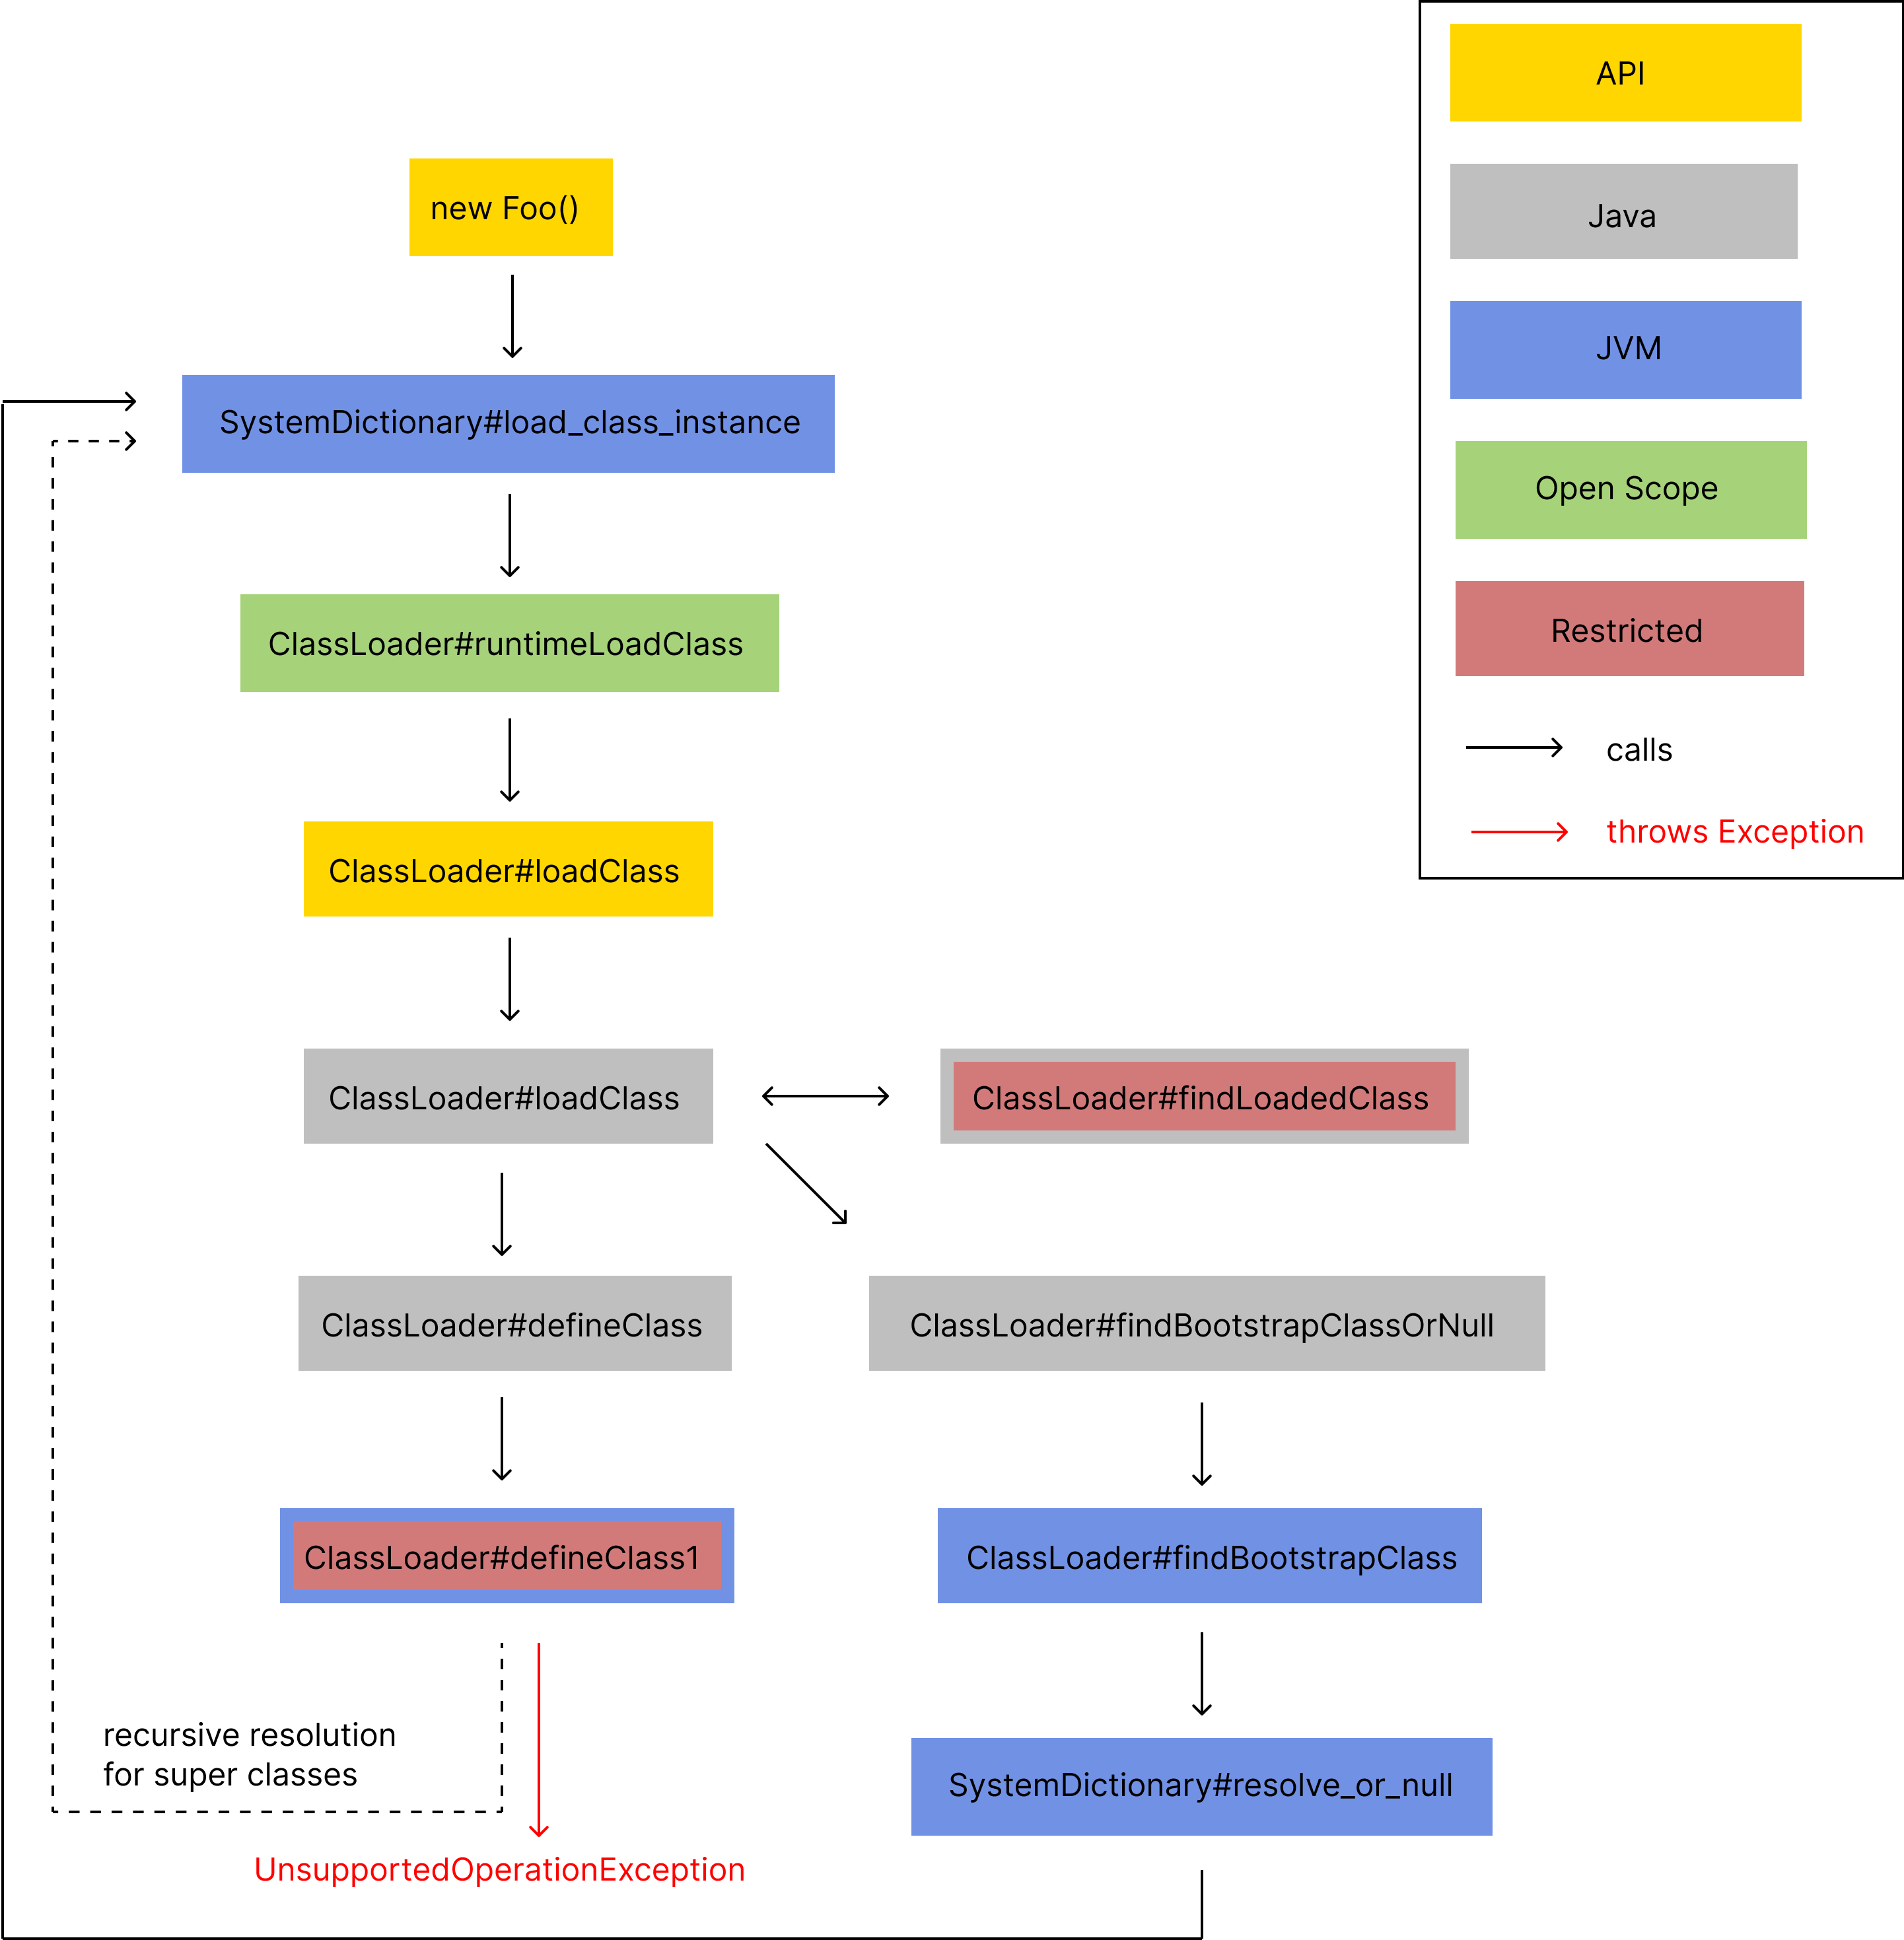
\includegraphics[scale=0.5]{resources/Group 403.png}
    \caption{Calling sequence for class loading, with the wrapper function \texttt{runtimeLoadClass} and scopes to support dynamic class loading at runtime.}
    \label{fig:load_class}
\end{figure}

Dynamic invocation required multiple design iterations to keep the changes to a minimum. Figure~\ref{fig:define_class_0} show all the entry points from which \verb|java.lang.ClassLoader#defineClass0| can be invoked to define a hidden class, and illustrates the final state of the design. For readability reason, the stack trace is not exhaustive and focuses on methods that lead to class definition and that have multiple callers.   
In the first implementation, scopes where open in \verb|java.lang.invoke.LambdaMetfactory| in both the \verb|metafactory| and the \verb|altMetafactory| methods, if the invocation was part of the \verb|invokedynamic| instruction.
This initial design had two issues. The first one being that it required us to check the stack trace and see if the \verb|java.lang.invoke.BootstrapMethodInvoker| was on the path to differentiate JVM from user calls. The second was that it was too restrictive, thus incorrect according to Native Image semantic, as the only bootstrap method that where allowed to be resolved at runtime where for lambda expressions.
Instead, we placed the scope lower on the stack trace, in the \verb|java.lang.BootstrapMethodInvoker#invoke| method. This method is invoked by the JVM in the process of linking the \verb|CallSite| to resolve (and invoke) the bootstrap method. The scope is open only for bootstrap methods that Native Image compiles at build time.
Figure~\ref{fig:define_class_0}, shows that moving the opening of the scope up or down on the stack trace would mean introducing an additional change because of the branching out. We also do not have the required metadata on the bootstrap method to place it in the JVM.   

Three main categories of user calls can result in the resolution of a method handle such that the JVM emits calls to define internal classes of the JDK at runtime: the invocation, and binding of a method handle and the lookup of an executable or field. As an optimization, the JVM compiles \verb|LambdaForm|, \verb|InjectedInvoker|, specialized \verb|BoundMethodHandle| and other automatically generated classes. 
In Native Image, these classes are either forced interpreted, or does not generate specialized code. Thus, letting Java under native restrictions define these classes does not contradict Native Image semantics. For performance reason, we decided to open scopes in the concerned methods, and let the JVM compile these forms at runtime.

\begin{figure}
    \centering
    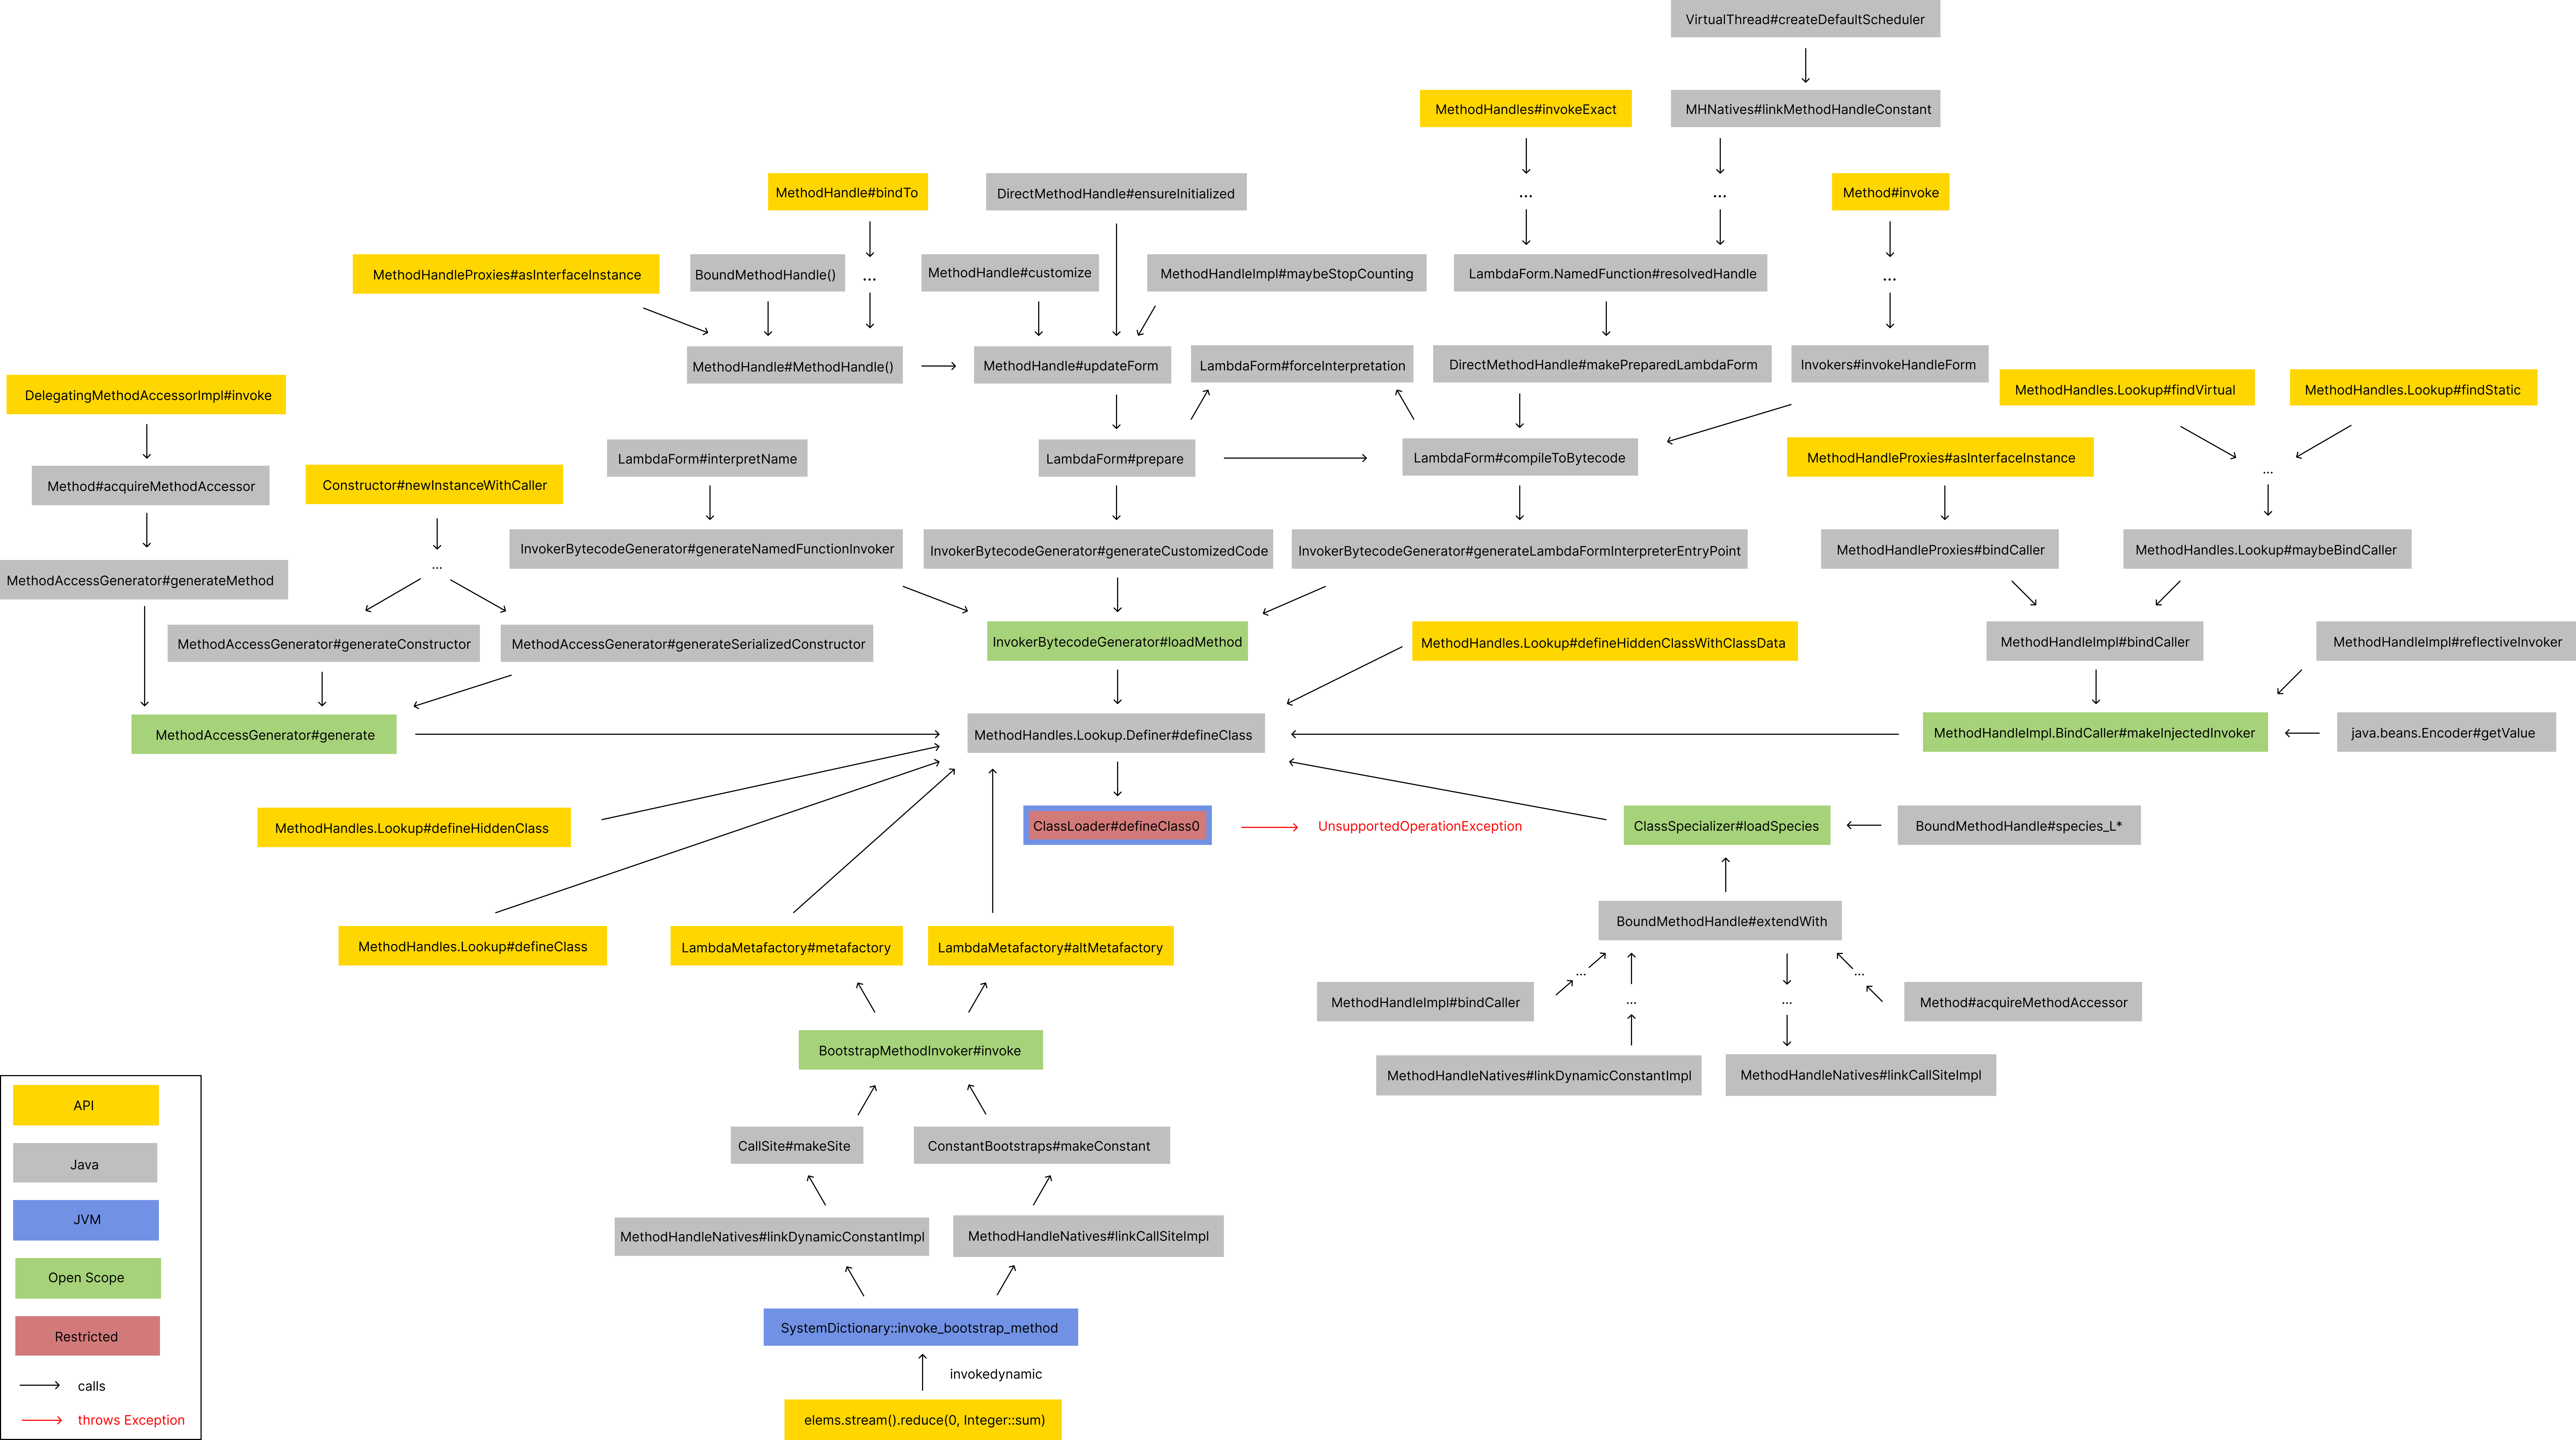
\includegraphics[angle=90,origin=c,scale=0.26]{resources/Group 401.png}
    \caption{Entry points for the method \texttt{java.lang.ClassLoader\#defineClass0}, with an abbreviated version of the stack trace.}
    \label{fig:define_class_0}
\end{figure}

Finally, \verb|defineClass1|, \verb|defineClass2| and \verb|defineClass0| are all native methods. Since the Java Native Interface~(JNI)~\cite{noauthor_jni_nodate} enables downcalls to the JVM's implementation of the define class method, we insert the native restrictions checks in the \verb|SystemDictionary::resolve_from_stream| which is part of the common code for \verb|JVM_DefineClass| and \verb|JVM_DefineClassWithSource|. If none of the scopes are open, the call will result in an \verb|UnsupportedOperationException|. 

%%%%%%%%%%%%%%%%%%%%%%%%%%%%%%%%
\subsection{Reflection}
%%%%%%%%%%%%%%%%%%%%%%%%%%%%%%%%
Designing Java under native restrictions for reflection consists in adding native restrictions checks to all methods in the \verb|java.lang.Class| class, the package \verb|java.lang.invoke.reflect|, and \verb|jdk.internal.sun.misc.Unsafe| that returns a reflectively-accessed element (see Section~\ref{native_image_specs} for a detailed list of the checks). 
If the reflectively-accessed element is not registered for reflection, a \verb|MissingReflectionRegistrationError| is thrown.

Similarly to reflection, \verb|java.lang.MethodHandles.Lookup| provides an API to look up \verb|Executables|, \verb|Fields|, and \verb|VarHandles|, and returns a method handle to access the element.
Internally the method handle contains a \verb|MemberName| that encapsulate all the element's metadata, that is it's declaring class, the element's name, and its type parameters if it has any. The \verb|MemberName| must first be resolved, in Native Image this is done with reflection.   
In Java under native restrictions we introduce a reflective access check in the method \verb|java.lang.invoke.MemberName#resolve|. As parts of the internal code for the tracing agent relies on lambda expressions to store the metadata, we also open a scope in \verb|MethodHandles#linkMethodHandleConstant| to break the loop.

% REST TO BE DETERMNINED....

%%%%%%%%%%%%%%%%%%%%%%%%%%%%%%%%
\section{Improving Usability}
%%%%%%%%%%%%%%%%%%%%%%%%%%%%%%%%
In this section, we will see how the Java mode fit in the overall Native Image usability plan. 

%%%%%%%%%%%%%%%%%%%%%%%%%%%%%%%%
\subsection{Quick turnaround for reachability metadata}
%%%%%%%%%%%%%%%%%%%%%%%%%%%%%%%%
One of the main goal of this thesis is to streamline reachability metadata computation for users.
The first step in the computation of these metadata is the collection. To achieve this Native Image offers a tracing agent that automatically collect the reachability metadata required for an application. This agent omits to log metadata for certain JDK internal classes (the \verb|MethodHandle| and its subtypes, classes from the \verb|java.lang| package, etc.), because Native Image does not require these elements to be registered, as the reachability of these elements can be proven in the code.  

To simplify the work flow and provide more transparency, we implement a tracing agent in the Java mode. In essence, the tracing agent is simply another language restriction added to the JDK. It is designed to follow the exact same path during an execution as Java under native restrictions. Instead of performing restriction checks, the agent logs the reflectively-accessed elements and outputs a configuration at the end of the execution run.
This also offers the advantage of giving a concrete list of JDK internal classes and methods that are proven in the code.

We propose a new and optimized workflow for computing metadata: (1) run the agent, (2) test the configuration with Java under native restrictions, (3.a) if the execution did not result in an exception build the \textit{native-image}, (3.b) otherwise debug the application by attaching a Java debugger.

%%%%%%%%%%%%%%%%%%%%%%%%%%%%%%%%
\subsection{Say Goodbye to GDB}
%%%%%%%%%%%%%%%%%%%%%%%%%%%%%%%%
Debugging is not an easy task. While it is possible to attach a java debugger to the image build process, debugging the image itself is trickier.

% -----------------------------------
% [Copy pasted from sacha]
% Debugging a compiler is not as straightforward as debugging most other types of projects. There
% are two different parts. The first easier one is debugging the image construction. As it is written in
% Java, it is possible to attach a Java debugger on the code and debug it as most other programs. The
% error messages are understandable and usually allow to quickly find the issue. The second one,
% consisting in debugging the image, is harder. While most error messages can still help identifying
% the cause of the failures, a lot of them end in a segmentation fault, meaning the best ally for
% debugging images is GDB and the assembly code obtained using objdump. Sadly, a lot of useful
% tools, such as valgrind, are not implemented for RISC-V yet. Since the backend works with other
% architectures, it is possible to compare the execution with another binary. The call trace is the
% same as it would be if the code was executed on the JVM, thus allowing to follow the execution
% through the Java source code. Usually, carefully looking at the registers and the memory during
% execution is enough to understand the problem and pinpoint the error.
% -----------------------------------

%%%%%%%%%%%%%%%%%%%%%%%%%%%%%%%%
\subsection{Defining expected behaviour}
%%%%%%%%%%%%%%%%%%%%%%%%%%%%%%%%
Our first approach to specifying Native Image semantic for reflection and dynamic class loading consisted in creating a Technology Compatibility Kit~(TCK). The TCK is a test suite that illustrates the specifications, it gives concrete examples of the expected behaviours, and provides a future-proof way of asserting that different versions of Native Image still behaves according to the same semantic.
It's designed to run with both Native Image and Java.

Tests harnesses usually use annotations to get the test classes and individual tests to run. JUnit's~\cite{noauthor_junit_nodate} \verb|@Test| annotation on methods, for example, can be reflectively queried to obtain the test \verb|Method| to invoke in the test harness.   
Since using reflection in the TCK to test reflection is not an option, we instead rely on an annotation processor, to generate on the fly all the data structure needed to run the test harness at compile time without using any reflective call (see Section~\ref{TCK} for details on the implementation). 

The TCK contains positive and negative unit tests for dynamic class loading, reflection and the security manager. To guarantee the correctness of the tests themselves, in particular for reflection, each test uses reflection on different dummy classes, such that the tests do not interfere with each other.
Despite - or thank to - its simplicity, the TCK did enable us to catch some bugs in Native Image.
Some were trivial, see Figure, as Native Image simply returned the wrong type of exception. 

Put list of bugs here!
This one does not throw:
public class Main {
    public static void main(String[] args) throws Exception {
        Class<?> cl = Class.forName("pfoo.PackageFoo");
    }
}

But then this one does
public class Main {
    public static String opaque(String s) {
        System.out.println();
        return s;
    }
    public static void main(String[] args) throws Exception {
        Class<?> cl = Class.forName(opaque("pfoo.PackageFoo"));
    }
}

This one does not throw:
package foo;
public class Foo {
    public String toString() {
        return "Hello There " + message;
    }
}
public static void testFindVirtual(MethodHandles.Lookup lookup) throws Throwable {
    String methodName = "toString";
    MethodHandle mh = lookup.findVirtual(Foo.class, hideLiterals(methodName), mt(String.class));
}
This one does
package foo;
public class FooLoader extends ClassLoader {
    @Override
    public Class<?> loadClass(String name) throws ClassNotFoundException {
        return super.loadClass(name);
    }
}
public static void testLoadClassBindCaller(MethodHandles.Lookup lookup) throws Throwable {
    MethodHandle mh = lookup.findVirtual(FooLoader.class, "loadClass", mt(Class.class, String.class));
}

Always hide the parameters behind a method call that can't be inlined or it doesn't throw


Defining class: Avoid bytecode rewriting -> create a loadClass wrapper instead, to differentiate users from the interpreters call
Balance between what needs to be changed in Native Image, driving the specs with this Java mode, and using part of what is in Nativ eImage in Java mode (e.g. 
MissingReflectionRegistrationError is still in progress in Native Image, but also using in Java).

Building the agent after doing the defineClass -> back and forth
SecurityManager was changed in Java moide, so had to change in NI, but other changes were made in NI so also had to propagate back the changes into the Java mode.
etc.


%%%%%%%%%%%%%%%%%%%%%%%%%%%%%%%%
\chapter{Implementation}
%%%%%%%%%%%%%%%%%%%%%%%%%%%%%%%%
% The implementation covers some of the implementation details of your project.
% This is not intended to be a low level description of every line of code that
% you wrote but covers the implementation aspects of the projects.
% Please provide as stable as possible links to the implementation source code.
A mix of software archeology and software surgery.
LanguageRestrictions, Restrictions bundles and restrictions


%%%%%%%%%%%%%%%%%%%%%%%%%%%%%%%%
\section{LanguageRestrictionManager}
%%%%%%%%%%%%%%%%%%%%%%%%%%%%%%%%
The LanguageRestrictionManager is the main entry point to the native restrictions. It provides a singleton instance of the abtract class LanguageRestriction.
The LanguageRestriction is subtyped by the NativeLanguageRestrion - by default models Native Image behaviour -, the NoLanguageRestriction - by default models Java semantics - and the NativeTraceLanguageRestriction, the JAva tracing agent that we implemented. 

It is also the interface for every native restrictions checks, and is used to hide away the scope abstraction when possible.

%%%%%%%%%%%%%%%%%%%%%%%%%%%%%%%%
\section{Native Restrictions Scopes and Checks}
%%%%%%%%%%%%%%%%%%%%%%%%%%%%%%%%
Concretely scopes are thread locals of integers, basically counters!
Each time a region is entered, the counter is incremented, and each time a region is left, the counter is decremented. This account for recursive calls (they either all get disabled or all enabled).

Put example code here.
\begin{lstlisting}[language=Java]
private Class<?> runtimeLoadClass(String name) throws ClassNotFoundException {
    try(ClassLoaderDefineClass unused = ClassLoaderLoaderDefineClass .setIsRuntimeDefineClassAllowed()) {
        return this.loadClass(name);
    }
}
\end{lstlisting}
To avoid memory leak, the thread local is instantiated in a try-catch clause, and implements the Autocloasable interface.
To minimize changes made to the JDK, the try catch clause is hidden in a Lambda whenever possible (i.e. StackOverflow can happen when the region is located in part of the JDK used to bootstrap lambdas).

%%%%%%%%%%%%%%%%%%%%%%%%%%%%%%%%
% \section{Dynamic Class Loading}
%%%%%%%%%%%%%%%%%%%%%%%%%%%%%%%%
% Native Image does not allow for runtime definition of classes that were not preloaded beforehand.
% To simulate this behavior, we introduce the wrapper method java.lang.ClassLoader#runtimeLoadClass. The only entry point for this private method is the interpreter. If not preloaded, then a class may be defined at runtime only if resolving the class or interface was required by one of the following instructions:
% anewarray, checkcast, getfield, getstatic, instanceof, invokedynamic, invokeinterface, invokespecial,
% invokestatic, invokevirtual, ldc, ldc\_w, multianewarray, new, putfield, and putstatic.
% The wrapper then dispatches the call to the method loadClass to the delegate class loader, as intended when running without restrictions.
% Runtime calls to the public method java.lang.ClassLoader#loadClass methods first checks if the class was preloaded (i.e. checking the inclusion of the class in the reflection metadata is sufficient to simulate Native Image behavior in this Java mode), before allowing it to be defined.

% \begin{lstlisting}[language=Java]
% private Class<?> runtimeLoadClass(String name) throws ClassNotFoundException {
%     try(ClassLoaderDefineClass unused = ClassLoaderLoaderDefineClass .setIsRuntimeDefineClassAllowed()) {
%         return this.loadClass(name);
%     }
% }
% \end{lstlisting}

% TODO add a simple running example: in one case creating an object new Foo() -> intepreter call
% in another loadong the class foo with and without preloading

% Do an upcall in native code in ClassLoader.c to check if the dynamicClassLoading is restricted or not and throw an UnsupportedOperationException is so.

%%%%%%%%%%%%%%%%%%%%%%%%%%%%%%%%
% \section{Invoke dynamic}
%%%%%%%%%%%%%%%%%%%%%%%%%%%%%%%%
% Talk about BMI, and how certain BMI are allowed and other not, as well as restricting the LambdaMetafactory
% Use lambda to surround and hide the checks

%%%%%%%%%%%%%%%%%%%%%%%%%%%%%%%%
% \section{Reflection}
%%%%%%%%%%%%%%%%%%%%%%%%%%%%%%%%
% don't want to trace internal classes!
% > first implementation of the restrict for LambdaMetafactory and the BMI was too restrictive,
% i.e. only allowed LambdaMEtfactory all other bsmethod where restricted, which is not correct ->
% checked NI and try to get as close as possible, it executes some safe bsmethods at build time and
% the rest is interpreted at runtime -> basically only lambda and other System class are allowed in
% Java mode, if the user tries to do something strange (assuming they haven’t overriden the App class
% loader), then either the call site must have been preloaded before, or it will throw when it tries to
% resolve the method name

%%%%%%%%%%%%%%%%%%%%%%%%%%%%%%%%
% \section{Tracing agent}
%%%%%%%%%%%%%%%%%%%%%%%%%%%%%%%%
% Have everything in one place -> simple work flow run the agent test with java under native restrictions adn then build the image -> don't need to build graalvm before
%%%%%%%%%%%%%%%%%%%%%%%%%%%%%%%%
% \section{Unimplemented feature: Security Manager}
%%%%%%%%%%%%%%%%%%%%%%%%%%%%%%%%
% -> Throws a VMError fatal error, cannot be catched
% -> instead

%%%%%%%%%%%%%%%%%%%%%%%%%%%%%%%%
\section{Technology Compatibility Kit}\label{TCK}
%%%%%%%%%%%%%%%%%%%%%%%%%%%%%%%%
An experience in meta-programming. 
Gradle project designed to compile with an annotation processor. Parses all @Test annotation and write the json configuration for each test on the fly
during compilation.
Test harness run all test that implements the TestProvider class. Single test per file
The reflection configurations are not on the classpath on purpose. There's a flag in NI and Java so that the path to the reflection configurations files can be specified.
-> Build two native images, one with the reflection and another without. Run with Java with and without the reflection configuration path specified as a sys prop.


%%%%%%%%%%%%%%%%%%%%%%%%%%%%%%%%
\chapter{The Native Image Specification}\label{native_image_specs}
%%%%%%%%%%%%%%%%%%%%%%%%%%%%%%%%
% https://pandoc.org/diagram.svgz?v=20240215100618
%% TODO add snippets of code to show how it differes from normal Java
# Native Image Semantics

Native Image operates under a closed-world assumption. This assumption affects the semantics of the 
Java® programming language as defined in the 
[Java Language Specification](https://docs.oracle.com/javase/specs/jls/se21/html/index.html).
We refer to this set of semantics as Native Image semantics, and is strictly equivalent to running
Java under native restrictions.

This document specifies the semantics of Native Image.
It is organised according to the following sections:
* [Reflection](#reflection)
* [Resources](#resources)
* [Serialization](#serialization)
* [Dynamic Class Loading](#dynamic-class-loading)
* [Misc.](#misc)

# Reflection
Under native restrictions, every reflectively-accessed element, that is `Class`, `Executable`, and `Field`, must 
be included in the reflection metadata (see [Specifying Reflection Metadata in JSON](https://www.graalvm.org/latest/reference-manual/native-image/metadata/#specifying-reflection-metadata-in-json)
for more details). If the element is not registered for reflection, then a `MissingReflectionRegistrationError` is thrown.

### Reflectively-Accessing a Class
Calling `java.lang.Class#forName` for a class or interface C requires C to be registered for reflection.
If C is registered, and C cannot be located, then a `ClassNotFoundException` is thrown. 
Superclasses of C are not automatically registered for reflection if C is registered.

Creating a new array of component type C using `java.lang.reflect.Array#newInstance` requires C to be 
registered for reflection.

Instantiating C with the method `sun.misc.Unsafe#allocateInstance` requires C to be 
registered for reflection and the flag `unsafeAllocated` must be set to true.

### Reflectively-Accessing a Method
Calling `java.lang.Class#getMethod` and `java.lang.Class#getDeclaredMethod` on a class or interface C for a method M, 
with parameters of types T<sub>1</sub>...T<sub>n</sub>, require C, M and T<sub>1</sub>...T<sub>n</sub> to be registered 
for reflection.
If M is registered, but M cannot be found, then a `NoSuchMethodException` is thrown.

Invoking the method M of C using `java.lang.reflect.Method#invoke` requires C to be registered for reflection
and M to be registered as accessed in the reflection metadata.
A `MissingReflectionRegistrationError` is thrown if C or M is not registered for reflection, or 
if M is only registered as being queried.

### Reflectively-Accessing a Constructor
Calling `java.lang.Class#getConstructor` and `java.lang.Class#getDeclaredConstructor` on a class or interface C 
for a constructor N with parameters of types T<sub>1</sub>...T<sub>n</sub>, require C, M and T<sub>1</sub>...T<sub>n</sub>
to be registered for reflection,
If N is registered, but N cannot be found, then a `NoSuchMethodException` is thrown.

Creating a new instance of the class or interface C using the constructor N using
`java.lang.reflect.Constructor#newInstance` requires C to be registered for reflection
and N to be registered as accessed in the reflection metadata.
A `MissingReflectionRegistrationError` is thrown if C or N is not registered for reflection, or
if N is only registered as being queried.

### Reflectively-Accessing a Field
Calling `java.lang.Class#getField` and `java.lang.Class#getDeclaredField` on a class or interface C for a field F,
require the C and F to be registered for reflection.
If F is registered for reflection, but F cannot be found, then a `NoSuchFieldException` is thrown.

### Reflectively-Accessing Member Classes and Interfaces
When called on the class or interface C, the following methods require C to be registered for reflection with
a specific flag set:
* `java.lang.Class#getClasses` along with the flag `allPublicClasses` set to true
* `java.lang.Class#getDeclaredClasses` along with the flag `allDeclaredClasses` set to true

### Reflectively-Accessing the Methods of a Class
When called on the class or interface C, the following methods require C to be registered for reflection with 
a specific flag set:
* `java.lang.Class#getMethods` along with the flag `allPublicMethods` set to true
* `java.lang.Class#getDeclaredMethods` along with the flag `allDeclaredMethods` set to true

### Reflectively-Accessing the Constructors of a Class
When called on the class or interface C, the following methods require C to be registered for reflection with
a specific flag set:
* `java.lang.Class#getConstructors` along with the flag `allPublicMethods` set to true
* `java.lang.Class#getDeclaredConstructors` along with the flag `allDeclaredMethods` set to true

### Reflectively-Accessing the Fields of a Class
When called on the class or interface C, the following methods require C to be registered for reflection with
a specific flag set:
* `java.lang.Class#getFields` along with the flag `allPublicFields` set to true
* `java.lang.Class#getDeclaredFields` along with the flag `allDeclaredFields` set to true

### Reflectively-Accessing the Permitted Subclasses of a Class
Calling `java.lang.Class#getPermittedSubclasses` on a class or interface C requires C to be registered for reflection
and its flag `allPermittedSubclasses` to be set to true.

### Reflectively-Accessing the Nest Members of a Class
Calling `java.lang.Class#getNestMembers` on a class or interface C requires C to be registered for reflection 
and its flag `allNestMembers` to be set to true.

### Reflectively-Accessing the Record Components of a Class
Calling `java.lang.Class#getRecordComponents`on a class or interface C requires C to be registered for reflection
and its flag `allRecordComponents` to be set to true.

### Reflectively-Accessing the Signers of a Class
Calling `java.lang.Class#getSigners`on a class or interface C requires C to be registered for reflection
and its flag `allSigners` to be set to true.

## Resources
## Serialization

## Dynamic Class Loading
In this section, we explain the differences that occur during the process of dynamically loading
a class or interface at runtime under native restrictions. 
If not explicitly specified, then a call to a method refers to a call from the API, 
rather than an internal calls.

### Class and Interface Resolution
Under native restrictions, the following rules apply: 
* All classes from the classpath are linked before the execution of the program
* All `invokedynamic` instructions are resolved at build time before program execution and replaced
  with adequate bytecodes

A class or interface dynamically loaded at runtime must be registered for reflection.

If the element is not registered, then:
* Calling any of the declared methods `loadClass` of `java.lang.ClassLoader` will result in a 
`MissingReflectionRegistrationError`.
* Calling any method of a user-defined class loader that depends on the methods `java.lang.ClassLoader#loadClass`, 
`java.lang.ClassLoader#findLoadedClass` or `java.lang.ClassLoader#findBootstrapClassOrNull` 
will result in a `MissingReflectionRegistrationError`.

If the element is registered, then resolution proceeds as described in 
[Section 5.4.3. of the JLS](https://docs.oracle.com/javase/specs/jvms/se21/html/jvms-5.html#jvms-5.4.3).

### Method Handle Resolution
Unless they are used as part of the `invokedynamic` instruction, calls to the following methods 
will result in an `UnsupportedOperationException`:
* `java.lang.invoke.MethodHandles.Lookup#defineClass`
* `java.lang.invoke.MethodHandles.Lookup#defineHiddenClass`
* `java.lang.invoke.MethodHandles.Lookup#defineHiddenClassWithClassData`

### java.lang.invoke.LambdaMetafactory
Unless they are used as part of the `invokedynamic` instruction, calls to `java.lang.invoke.LambdaMetafactory#metafactory` 
and `java.lang.invoke.LambdaMetafactory#altMetafactory` will result in an `UnsupportedOperationException`.


## Unimplemented Features
#### java.lang.SecurityManager
The `java.lang.SecurityManager` behaves in the following ways:
* `java.lang.System#getSecurityManager()` always returns `null`
* `java.lang.System#setSecurityManager(SecurityManager sm)` returns without exception if `sm` is null. 
It throws a `SecurityException` if the system property `java.security.manager` is not set to `disallow`, and an 
`UnsupportedOperationException` otherwise.



%%%%%%%%%%%%%%%%%%%%%%%%%%%%%%%%
\chapter{Evaluation}
%%%%%%%%%%%%%%%%%%%%%%%%%%%%%%%%
JCK and TCK as testing frameworks
% In the evaluation you convince the reader that your design works as intended.
% Describe the evaluation setup, the designed experiments, and how the
% experiments showcase the individual points you want to prove.


design flaw, when overloading the classloader, there's currently no way of knowing if a check has already been made for a class or not -> we check the metadata each time defineClass or findLoadedClass is called

benchmarks
